\chapter{Systemadesign}\label{Systemdesign}
Systemdesignet beskriver hvordan PC Applikation er opbygget og hvordan PC Apllikations klasser integrerer med hinanden.  

Nedenfor vil relevante diagrammer blive gennemgået. For detaljeret gennemgang af systemdesign for Automatisk Ultralydsscanner se Bilag  \ref{Udviklingsdokument} Udviklingsdokument.

\section{Klassediagram}
Klassediagrammerne viser strukturen
i systemet og deres relationer. Hver klasse indeholder de vigtigste metoder og attributer
i klassen, der udgør funktionaliteten i PC Applikation. 

\subsection{GUI}
GUI-klassen Figur \ref{class_gui} indeholder brugergrænsefladen for PC Applikation.

\let\labelitemi\labelitemii
\begin{itemize}
\item{MainWindow}\newline
Giver anledning til at foretage et 3D scan. Såfremt en 3D scanning er gennemført giver det også anledning til at starte en ultralydsscanning.
Når menuen startes, oprettes en instans af RoboMaster, for at sætte Robotarm i standard positur. Dette er nødvendigt, hvis Robotarm skulle være i vejen for en 3D scanning.
Hvis der ikke er nogen forbindelse til Robotarm vil der 

\item{3DScanMenu}\newline
I denne menu er der mulighed for at se det nuværende dybdebillede, afgrænse området der skal 3D scannes og foretage en 3D scanning.

\item{UltrasoundScanMenu}\newline
I denne menu kan den procentvise færdiggørelse af ultralydsscanningen følges. Der er også mulighed for at pause samt afbryde ultralydsscanningsprocessen.
\end{itemize}

\begin{figure}[H]
    \centering
    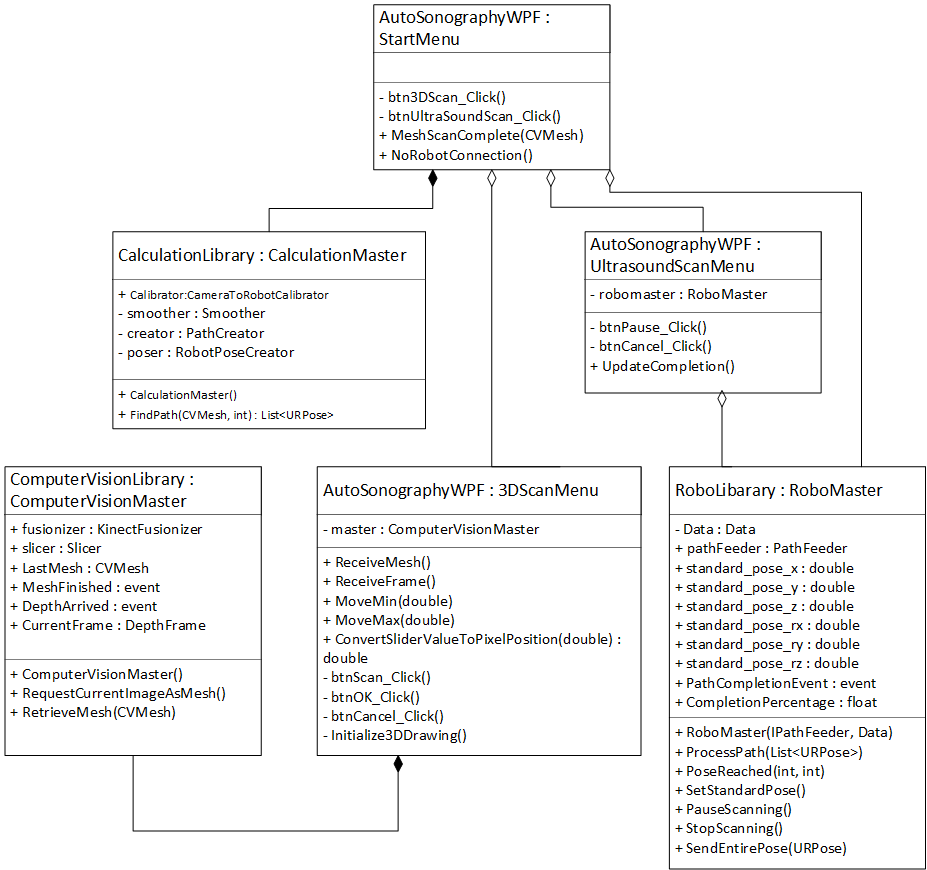
\includegraphics[width=1\textwidth]{figurer/d/Design/Class/uml_class_gui}
    \caption{Klassediagram for GUI}
    \label{class_gui}
\end{figure}

